\documentclass{article}


\PassOptionsToPackage{numbers, compress}{natbib}
\usepackage[preprint]{neurips_2020}
    
\usepackage[utf8]{inputenc} % allow utf-8 input
\usepackage[T1]{fontenc}    % use 8-bit T1 fonts
\usepackage{hyperref}	    % hyperlinks
\usepackage{url}	    % simple URL typesetting
\usepackage{booktabs}	    % professional-quality tables
\usepackage{amsfonts}	    % blackboard math symbols
\usepackage{nicefrac}	    % compact symbols for 1/2, etc.
\usepackage{microtype}	    % microtypography
\usepackage{xcolor}	    % text color
\usepackage{xspace}
\usepackage{amsmath}
\usepackage{amssymb}
\usepackage{graphicx}
\usepackage{caption}
\usepackage{subcaption}

% YZ: does this title work? feel free to change lol
\title{Collaborative Filtering for Music Recommendation}

% The \author macro works with any number of authors. There are two commands
% used to separate the names and addresses of multiple authors: \And and \AND.
%
% Using \And between authors leaves it to LaTeX to determine where to break the
% lines. Using \AND forces a line break at that point. So, if LaTeX puts 3 of 4
% authors names on the first line, and the last on the second line, try using
% \AND instead of \And before the third author name.

\author{
  Zander Meitus \qquad Yiming Zhang \\
  University of Chicago \\
  \texttt{\{zmeitus,yimingz0\}@uchicago.edu}
}

\newcommand{\aoty}{{\bf AOTY}\xspace}
\DeclareMathOperator{\X}{\mathit{X}}
\DeclareMathOperator{\U}{\mathcal{U}}
\DeclareMathOperator{\I}{\mathcal{I}}
\newcommand{\card}[1]{\ensuremath{\lvert {#1} \rvert}}
\newcommand{\easer}{$\text{EASE}^\text{R}$\xspace}
\newcommand{\userknn}{UserKNN\xspace}
\newcommand{\norm}[1]{\ensuremath{\lVert #1 \rVert}}
\newcommand{\transpose}[1]{{#1}^\mathsf{T}}
\newcommand{\yiming}[1]{\textcolor{violet}{[#1 ---\textsc{YZ}]}}
\newcommand{\zander}[1]{\textcolor{blue}{[#1 ---\textsc{ZM}]}}
\newcommand{\secref}[1]{\S\ref{#1}}

\begin{document}

\maketitle

\section{Introduction}

In this project, we study music recommendation using tools we learned in the
 class and collaborative filtering (CF) methods.
Collaborative filtering performs matrix completion by leveraging user-level and
 album-level similarities: for a set of $n$ users and $p$ items, the user-item
 matrix $\X$ takes the form of $\X = \mathbb{R}^{n \times p}$, with potentially
 missing values when no rating is available.
Then, the recommendation problem boils down to identifying a set of ``good''
 items $\I_i$ for a user $i \in [n]$.

To study the problem of music recommendation, we create a new dataset \aoty as
 a testbed for music recommendation.
We chose to experiment with two recommendation algorithms,
 \easer~\citep{steckEmbarrassinglyShallowAutoencoders2019} and
 \userknn~\citep{resnickGroupLensOpenArchitecture1994}, for their
 state-of-the-art performance and computational tractability demonstrated by a
 recent survey~\citep{anelliTopNRecommendationAlgorithms2022}.
After implementation, we evaluate their performance on \aoty.
Both \easer and \userknn show strong recommendation performance: In a retrieval
 setting, \easer achieves an F1@20 score of 27.0, an impressive score
 considering there are over 8k potential albums.
In a classification setting, \userknn achieves an F1 of 82.2 on heldout
 user-item predicitions.

\section{Literature Review}
Collaborative filtering recommendation systems have been a major focus of
 machine learning for several decades, with applications in commerce,
 entertainment, professional networking and beyond \zander{add citations}.
In recommendation settings, observations for a given user are often sparse, and
 the model is tasked with predicting user preferences without much training data
 for the particular user.
There are a variety of model families that are well-suited to this task,
 including neighborhood-based, linear, matrix factorization, and neural models,
 among others \citep{anelliTopNRecommendationAlgorithms2022}.
Beyond computational complexity and performance on a given task, the model
 families differ in the types of tasks they are most adept at handling.
For example, some algorthmic families are better at handling implicit feedback
 datasets (where a value of 1 indicates a user interaction and a 0 indicates no
 user interaction), while others handle explicit feedback (where a user gives an
 item a rating on an ordinal or continuous scale)
 \citep{steckEmbarrassinglyShallowAutoencoders2019}.

As \citet{Schedl2018} illustrate, recommendation for music has unique
 differences from other recommendation tasks.
Individual songs last minutes, while other common recommendation items like
 movies or books are consumed over a much longer time period.
Songs are consumed sequentially, where the particular order is meaningful.
A given music catalog may contains tens of millions.
Schedl et.
al. argue that because of music's unique attributes, it is
worthwhile
studying recomendation systems when applied to music
in isolation \citep{Schedl2018}.

Our study is unique from existing music recommendation systems work both in its
 application and the dataset.
Our unit of recommendation is an album, while most commercial music
 recommendation systems operate at the song level \citep{Schedl2018}.
This distinction is important in an era where music critics and fans bemoan how
 the "endless mix-tape" of song recommendation algorithms detracts from the
 experience of listening to an album from start to finish
 \citep{toth2018,hilton2013}.
The dataset we've compiled and curated from \url{aoty.org} provides explicit
 feedback from users at the album level, which enables us to research
 performance differences in models intended for explicit and implicit feedback.

\section{Method}
Collaborative Filtering, the technique of inferring the preferences of one user
 using known information about other users, is the dominant class of algorithm
 for recommendation systems.
In this project, we plan to implement, extend and evaluate two CF algorithms,
 \easer and \userknn, demonstrated as among the state-of-the-art in a
 comprehensive survey by \citet{anelliTopNRecommendationAlgorithms2022}.

\paragraph*{\easer.}
\easer~\citep{steckEmbarrassinglyShallowAutoencoders2019}
is a linear model parameterized by a item-item matrix $B \in
	\mathbb{R}^{p \times p}$.
The weights $B$ are optimized with respect to the simple objective
 \begin{equation} \min_B \norm{\X - X B}_F^2 + \lambda \cdot \norm{B}_F^2
 \text{.
}
\end{equation}
Intuitively, \easer reconstructs user preferences using information about items
 exclusively.
In addition, \easer adds an matrix norm penalty, encouraging $B$ to be
 low-rank.
$B$ admits a degenerate solution $B = I$, under which the
recommendation system always recommends items that the user likes.
To avoid this solution, the author added an additional constraint that
 $\mathrm{diag}(B) = \mathbf{0}$.
Learning the weights of $B$ is a (constrained) convex optimization problem, and
 the optimal solution is given by  \begin{equation} \hat{B}_{i, j} =
	 \begin{cases} 0 & \text{if $i = j$} \\ -\frac{\hat{P}_{i, j}}{\hat{P}_{j, j}} &
               \text{otherwise,}     \\\end{cases} \end{equation} where $\hat{P} =
	 (\transpose{X} X + \lambda I)^{-1}$.

Despite its simplicity, computing this closed-form solution requires inverting
 an $p \times p$ matrix, taking $\mathcal{O}(p^3)$ time in a typical commercial
 implementation.
To save computational cost, we experiment with mini-batch stochastic gradient
 descent as an alternative technique for computing $\hat{B}$.
To compute the loss $\norm{\X - X \hat{B}}_F^2 + \lambda \cdot
	 \norm{\hat{B}}_F^2$, we need to multiply a sparse matrice $X$ with $B$, which
 can be computed in $\mathcal{O}(x p)$ time, where $x$ is the number non-zero
 elements in $X$.
Then, this alternative training procedure takes $\mathcal{O}(kxp)$ time, where
 $k$ is the number of iterations until convergence.

\paragraph*{\userknn.}
Neighborhood-based recommendation methods essentially treat the preference of a
 user $u$ as a weighted sum of preferences of other users under some notion of
 similarity.
For a pair of users $u, v$,
 \userknn~\citep{resnickGroupLensOpenArchitecture1994} measures the similarity
 between users with the correlation coefficient $r_{uv}$ between items that $u$
 and $v$ both rated.
The predicted score for an item is the weighted sum of ratings of similar
 users, after adjusting for the ``baseline rating'' that the user gives to an
 average item.
\begin{equation}
P = \vec{\mu} + \frac{(A - \bar J)R}{M \card{R}} \end{equation}  $P$ is
 prediction matrix of $n$ albums and $p$ users.
$\mu$ is the average
rating
of each reviewer. $A$ is the provided $n \times p$ ratings matrix. $\bar J$ is
an $n$
by $p$
matrix where the $i,j$ entry is the average rating of the $j$th reviewer,
exluding the $i$th
rating. $R$ is the reviwer correlation matrix with its diagonal set to 0. $M$
is
a mask of
$A$, where cells with ratings in $A$ are $1$ in M, and all other values of $M$
are 0.
The approach is non-parametric in that there is no loss function to optimize
 for and no parameters to tune.
The algorithm simply aggregates known user data to produce predictions.
It is important to note that is this setting, the $n$ albums are the matrix
 rows, while the $p$ users are the columns, which is the reverse of the \easer
 setup.

\section{Experimental Setup}
\label{sec:setup}
\paragraph*{Data curation.}
For this project, we have created a dataset of album reviews, named \aoty, by
 scraping data from \url{https://aoty.org}.
On this website, users create profiles and rank albums from 0 to 100.
After filtering out albums with $<100$ total reviews and users with $<10$
 positive reviews, \aoty has a total of $8,855$ albums and $22,167$ users.
The average album in the dataset has $426.8$ reviews.
The user-album matrix is very sparse: for \aoty, the sparsity $s = 1.9 \times
	 10^{-2}$.
The {\em data sparsity} problem~\citep{suSurveyCollaborativeFiltering2009} in
 the user-item matrix is a major challenge in most real-world recommendation
 problems, and we believe this property makes \aoty a suitable testbed for
 studying recommendation.

\paragraph*{Evaluation setup and metrics.}
\easer assumes {\em implicit feedback}, where interactions are binary
labels indicating whether user likes an item or not.
Therefore, we binarize the \aoty dataset by considering all reviews with rating
 $\ge 75$ as the positive class, and all other reviews as the negative class.
In a {\em strong generalization} setting (i.e., testing on heldout users in
 training), we measure the performance of \easer on three common retrieval
 metrics.
Precision @ $k$ measures the percentage of recommended items that a user likes
 in top-$k$ recommendations, and recall @ $k$ measures the the coverage of all
 items liked by a user in top-$k$ recommendations.
F1 is defined as the harmonic mean of precision and recall.
Beyond these common retrieval metrics, we further consider the following
 metrics following \citet{anelliTopNRecommendationAlgorithms2022}:
 \begin{itemize} \item {\em Item Coverage}: Item Coverage (IC) measures the
 percentage of items that is recommended to at least one user.
\item {\em Gini}: Gini coefficient of the distribution of recommendation
measures its inequality.
\end{itemize}

\userknn takes {\em explicit feedback} (ratings) as input and generates
explicit ratings as output,
so we evaluate the model on mean absolute error (MAE) and root mean squared
error (RMSE).
We also convert the true and predicted ratings to implicit feedback following
 the same procedure as for \easer and evaluate on previously discussed retrieval
 metrics.
Since evaluation with \userknn is slow, we randomly selected 10 users in the
 test set for evaluation under the {\em strong generalization setting}.
We further report performance in the {\em weak generalization} setting, where a
 random sample of 20\% of ratings are omitted from the user-rating matrix $X$ to
 create a user-rating matrix $X^{\prime}$.
The algorithm is then run on $X^{\prime}$ to generate predictions.
The predictions for the omitted ratings are then compared to the true ratings
 to evaluate performance.
%  We evaluate \userknn in the weak generalization setting on the full user-rating
%  matrix, omitting a random sample of 20\% of the ratings for a total of 736,944
%  test predictions.
% We also evaluate \userknn in the strong generalization setting.
% To apply strong  generalization to \userknn, a new rating matrix needs to be
%  generated for each test user that is $n$ by $v$, where $v$ is the number of
%  valid ratings provided by the user.
% In each column, one of the valid values is omitted so that the predicted value
%  is not included in the correlation between the test user and all training
%  users.
% A correlation matrix $R_j$ for the $j$ test user then needs to be calcualted
%  between each column vector of the $j$th test user's matrix and the training
%  matrix $A$.
% Because this is computationally expensive to regenerate the correlation matrix,
%  we used only 10 random test users to evaluate \userknn in the strong
%  generalization setting with a total of 1,121 predicted ratings.

\section{Results}

\begin{figure*}[h]
	\centering
	\begin{subfigure}[b]{0.4\textwidth}
		\centering
		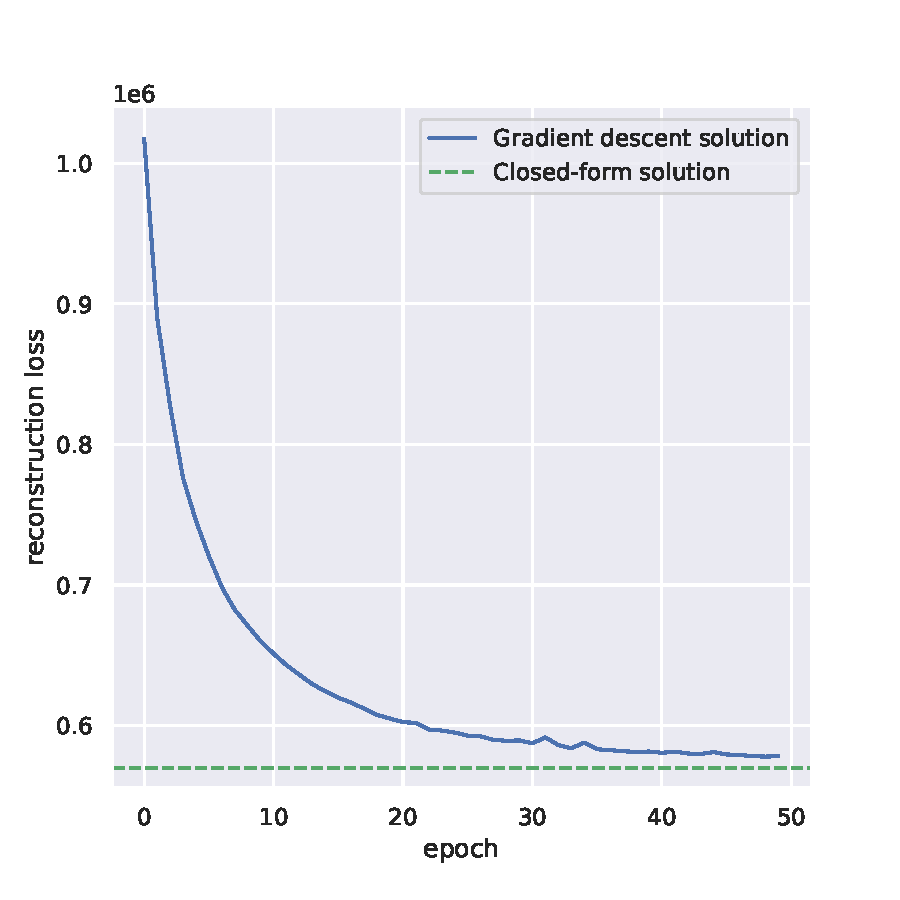
\includegraphics[width=\textwidth]{figures/recon-loss.pdf}
		\caption{Convergence of stochastic gradient descent (blue) to
			the optimal,
			closed-form solution (green) in \easer.}
		\label{fig:convergence}
	\end{subfigure}
	\hspace{0.1\textwidth}
	\begin{subfigure}[b]{0.4\textwidth}
		\centering
		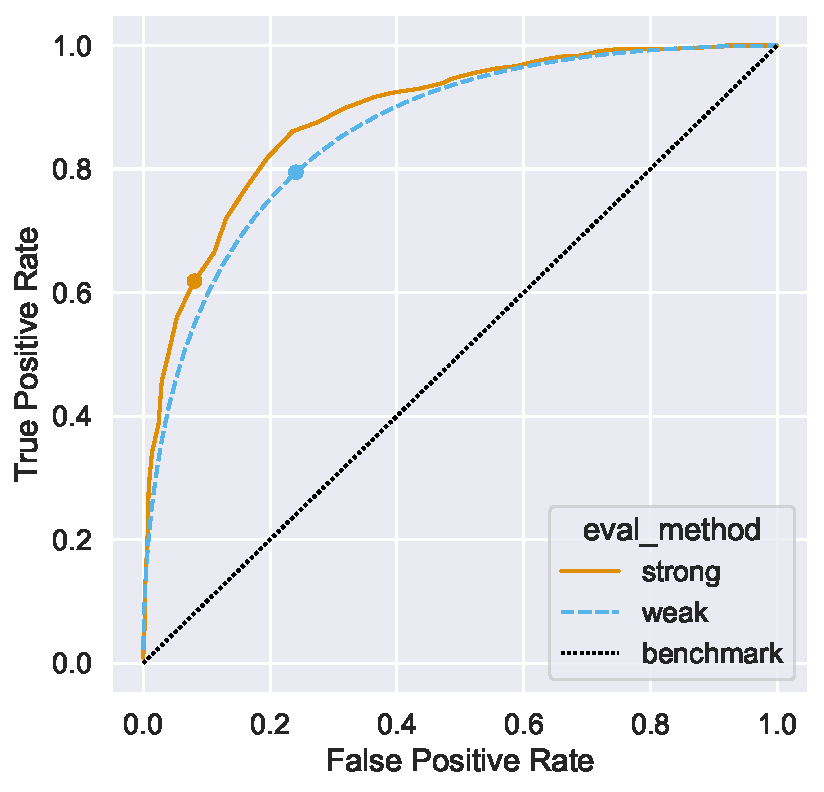
\includegraphics[width=\textwidth]{figures/user_knn_roc.pdf}
		\caption{\userknn performance on different implicit feedback
			thresholds.
			Dots represent evaluated threshold.
		}
	\end{subfigure}
	\caption{}
	\label{fig:1}
\end{figure*}

\begin{table*}[h]
	\centering
	\begin{tabular}{@{}llll@{}}
		\toprule
		Evaluation metrics @ $20$     & \easer (closed-form) & \easer
		(SGD)
		\\ \midrule
		Precision $\uparrow$          & $69.2$               & $69.2$
		\\
		Recall	$\uparrow$              & $21.0$               &
		$21.0$
		\\
		F1	$\uparrow$                  & $27.0$               &
		$27.0$
		\\
		Item Coverage	$\uparrow$       & $34.7\%$             &
		$34.7\%$
		\\
		Gini	$\downarrow$              & $0.925$              &
		$0.925$
		\\
		Optimization time	$\downarrow$ & 5 seconds
		                              & 107 seconds
		\\ \bottomrule
	\end{tabular}
	\caption{Evaluation of top-20 recommendations of \easer on a heldout
		test set. $\uparrow$ means higher is better, and $\downarrow$
		means
		lower is better.}
	\label{tab:easer-results}

\end{table*}

\paragraph*{\easer.}
We evaluate the both the closed-form version of \easer and our proposed
 stochastic gradient descent (SGD) approach on a heldout out test set of users.
We are interested in quantifying the recommendation quality of both algorithms,
 and understanding whether our proposed approach produces a solution that
 converges to the closed-form solution.

One way to understand the convergence behavior of the algorithm is by measuring
 the reconstruction loss $\norm{X - X \hat{B}}_F^2$.
In Figure \ref{fig:1}\ref{sub@fig:convergence}, we plot the reconstruction loss
 corresponding to $\hat{B}^{(t)}$, the weights at epoch $t$, against the epoch
 number $t$.
The green line corresponds to the reconstruction loss of the optimal
 closed-form solution.
We find that the reconstruction loss of stochastic gradient descent indeed
 converges to that of the closed-form solution.
This observation isn't surprising given that \easer has a convex objective, and
 gradient descent provably converges for convex optimization problems.
That said, SGD-based optimization takes 107 seconds in our experiment, 21x
 longer than that of computing the closed-form solution directly.
We suspect that although our proposed solution has smaller big-$\mathcal{O}$
 complexity on paper, it's not well-tuned compared  NumPy's matrix inversion
 algorithm.
In addition, unlike normal matrix multiplication, sparse matrix multiplication
 does not take advantage of memory locality, a hardware level optimization that
 makes sequential memory access fast.

\easer shows strong recommendation performance when evaluated on unseen users
in training, highlighted by a Precision @ $20$ score of $69.2$, meaning users
provided
positive reviews for the majority of items we recommended.
While the Recall @ $20$ score is only $21.0$, the cutoff of 20 items is less than the
 average number of reviews per user, making a perfect score unattainable.
We also argue that precision is the more relevant metric in
 recommendation, as we care mostly about recommending some, rather than
 all, items that a user will like.
We observe significant concentration in the recommendations of \easer, with
 roughly one-third of all albums recommended to at least one user.
The Gini score of $0.925$ highlights a strong inequality in the recommendation,
 with a small subset of albums being heavily favored over the rest.

\begin{table*}[h]
\centering
\begin{tabular}{@{}llll@{}}
\toprule
Evaluation metrics    & \userknn - Weak Gen. & \userknn -
Strong Gen.
\\ \midrule
Number of Ratings			  & 736,944
& 1,121 \\
Precision $\uparrow$	      & $85.1$		     & $85.0$
\\
Recall	$\uparrow$		& $79.5$	       & $62.4$
\\
F1	$\uparrow$		    & $82.2$		   &
$72.0$
\\
AUC $\uparrow$					& $86.1$
& $88.7$
\\
Mean Abs.
Error $\downarrow$	   & $8.55$		& $8.17$ \\ RMSE $\downarrow$ &
 $11.8$ &$10.7$ $0.925$ \\ Optimization time $\downarrow$ & 5 seconds & 107
 seconds \\ \bottomrule \end{tabular} \caption{Evaluation of \userknn on a
 heldout test set in weak generalization setting.
$\uparrow$ means
higher is better, and $\downarrow$
means lower is better.}
\label{tab:userknn-results}

\end{table*}

\paragraph*{\userknn.}
We evaluate \userknn in both a weak generalization and strong generalization
 setting, utilizing both the original explicit feedback ratings and engineered
 implicit feedback.
The weak setting included 736,944 test predictions sampled
 randomly across all users and albums, while the strong setting involved just 10
 randomly sampled users across all albums for a total of 1,121 test predictions.

The algorithm performs strongly in both the weak and strong generalization
 settings, with mean absolute error of 8.55 and 8.17 respectively.
To evaluate the model's performance on implicit feedback data, all true ratings
 $\geq$ 75 were converted to 1, while all other ratings were converted to 0.
Model predictions were also converted using the same threshold, though the ROC
 curve in figure X shows strong performance across different thresholds for
 model predictions with AUCs of 86.1 and 88.7 respectively.
At the selected threshold, the model has comparable recall in the weak and
 strong settings at 85.1 and 85.0, but the model has better recall in the weak
 setting.
This could be due to the small sample size in the strong setting or the
 threshold selection.

\newpage
\bibliography{ref,yiming}
\bibliographystyle{abbrvnat}
\end{document}